\chapter{Requirements}
\label{chapter:requirements}

The locking manager Warlock was created to replace the existing lock manager
which was a single point of failure in the system. To explore the need for
Warlock and to understand its requirements, we look at the architecture of
the system and the derived requirements for Warlock in this chapter.

Magic Land \citep{magicland} is a social%
\sidenote[2]{
  A social game usually runs on a ``social network'' and allows in-game
  interaction with other users on the same network.
}
resource management game by Wooga%
\sidenote[5]{
  Wooga \citep{wooga} is a games company developing games on social networks
  and mobile platforms.
}
. The game is used by hundreds to thousands of users everyday resulting in
thousands of \abbr{HTTP} requests every second. 90\% of these requests are
writes. This requires the back end%
\sidenote[7]{
  Back end is the part of the system that handles all the user's actions and
  state and is not directly accessed by the user.
}
handle lot of requests that are not cacheable. Traditional solutions which
involves using stateless servers for application management and all state
managed
by databases is not feasible for this access pattern. This let to the creation
of the architecture comprising of stateful servers that handled all the user
state changes and used database only for long term storage.

The system consists of the following components as shown in the figure
\figureref{magic.land.architecture}.

\begin{figure}
  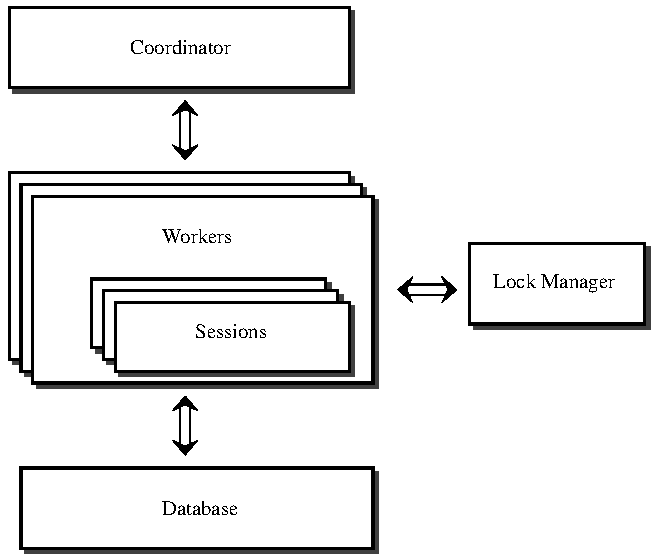
\includegraphics[width=0.6\wholewidth]{magic-land-arch}
  \caption[Magic Land Architecture]{%
    The figure depicts the high level view of the Magic Land system
    architecture.}
    \label{figure:magic.land.architecture}
  \normalcaption
\end{figure}

\begin{itemize}
    \iterm{Database}: The database is a persistent store used to store the 
    user's session information for long periods when the user is offline.
    \iterm{Worker}: User sessions are run on the worker. Each user session
    consists of an stateful Erlang process that handles all the requests
    generated by the user for that specific session.
    \iterm{Coordinator}: The coordinator decides on which worker a user's
    session need to be started on.
    \iterm{Lock Manager}: Strictly one session of the user needs to be
    running at any given point in order to avoid creating conflicting states.
    This is done by using a lock service that needs to be checked before
    starting a new user session.
\end{itemize}

A typical user flow consists of the user trying to load the game. The request
is sent to the coordinator which locates a suitable worker and asks it to
start the session for the given user. The worker tries to create a lock on
the users session by making a call to the lock manager with the user's id.
On successful lock, the worker loads the user's state from the database and
notifies that it is ready to accept requests.

The lock manager used is Redis \citep{redis}%
\sidenote[-3]{
  Redis is a performance oriented key-value store with support for multiple
  data structures and atomic primitives.
}
. The worker uses the Redis command \abbr{SETNX}%
\sidenote{
  \texttt{SETNX key value} - is a command that sets the \texttt{key} to hold
  \texttt{value} in a hash table only if \texttt{key} does not already exist
  in the table.
}. This makes sure that the worker can only start a new session if one is
not already running. Redis also supports asynchronous replication allowing the
data to be available in multiple locations.

While Redis is an excellent solution to the problem, it also becomes a single
point of failure for the entire system since no new sessions can be created in
the system if it is down. The goal of this thesis project is to try and replace
Redis as a locking system while being fault tolerant.

From the above background, we can now elaborate the system requirements:

\section{Key value store}
\label{section:ml.kv.store}

\req{The system should act as a key value store.}

The user is referenced across the system uniquely using a numeric user id
(\abbr{UID}). The user's session present in any of the workers can be uniquely 
referenced across all the workers uniquely using the session's process id
(\abbr{PID}).
The \abbr{UID} maps to \abbr{PID} and this mapping is stored in the lock
manager. To support this, the lock manager should support the hash
table primitives.

\section{Strong Consistency}

\req{All processes accessing the system should see the same results.}

The lock manager will be accessed by multiple workers concurrently. This
requires the manager to provide a consistent view to all the workers in
order to avoid session duplication.

Without strong consistency, it is possible that multiple divergent user states
exist at the same time. It might be possible to merge these states within
acceptable limits of effort.

\section{Maximize Availability}

\req{The system should target for maximum possible availability.}

Any downtime of the lock manager will translate to the game being unavailable
for a lot of users. The manager should target for high availability.

\section{High Read to Write Ratio}
\label{section:req.read.write.ratio}

\req{The manager should be designed and optimized to handle large read to write
ratio.}

The \abbr{UID} to \abbr{PID} mapping is read by multiple workers many times
during the life
of a user session as compared to writes which happen only when the user tries
to login. This means that the system can be optimized to maximize reads when
compared to writes.

\section{Dynamic Cluster}
\label{section:req.dynamic.cluster}

\req{It should be possible to add/remove nodes from the system as long as a
certain minimum number of nodes are available.}

Individual servers within a distributed system are susceptible to failures.
It should be possible to replace the failed servers without being forced
to restart the system.

As the number of users in the game grows, so does the number of requests to
the back end. The system should be able to handle additional load by allowing
addition of nodes dynamically.


\section{Masterless / System with Master Election}

\req{The system should not have a single point of failure.}

The system should not use special nodes whose failure can lead to the
entire system being out if service.

\section{Fault / Failure Tolerant}

\req{The system should handle node failures gracefully.}

Server failures in the system should be handled without affecting the service.
Individual failures should not cascade to rest of the system.

\section{Key Expiry}

\req{It should be possible to expire keys after a certain amount of time.}

The system should support the primitive that expires (deletes) the keys after
the specified time. This feature allows us to clear the system even in case
the worker missed it during session cleanup.

\section{Simple API}

\req{The system should have a simple \abbr{API}.}

The system should have a simple interface and should be simple to communicate
with.

\section{Programming Language Support}

\req{The system should be written in Erlang.}

Almost the entire back end stack of Magic Land is written in Erlang. Having the
lock manager also implemented in Erlang will allow it to communicate with
existing system in a more robust manner.

\section{Performance}

\req{The system needs to have high throughput.}

The system needs to be able to provide high throughput required to handle
millions of users.

